% Compile with XeLaTeX or LuaLaTeX (fontspec is used for IPA/Greek glyphs).
%   latexmk -xelatex main.tex      (or use Overleaf with the XeLaTeX compiler)
\documentclass[conference]{IEEEtran}

\usepackage{graphicx}
\usepackage{booktabs}
\usepackage{amsmath,amssymb}
\usepackage{fontspec}
% Font with broad IPA + Greek coverage for the few phonetic examples.
% Prefer the bundled DejaVuSans.ttf (works with tectonic and Overleaf alike),
% then a system-installed "DejaVu Sans", then fall back to the main font so the
% document always compiles.
\IfFileExists{fonts/DejaVuSans.ttf}
  {\newfontfamily\ipafont[Path=fonts/]{DejaVuSans.ttf}}
  {\IfFontExistsTF{DejaVu Sans}{\newfontfamily\ipafont{DejaVu Sans}}{\let\ipafont\relax}}
\newcommand{\ipa}[1]{{\ipafont #1}}
\usepackage[hidelinks]{hyperref}

\begin{document}

\title{LoRA for Multilingual Grapheme-to-Phoneme Conversion: Parameter-Efficient Adaptation of ByT5-G2P on Romanian and Modern Greek}

\author{\IEEEauthorblockN{Dan-Gabriel Tudor, \c{S}tefan-Rare\c{s} Stoian}
\IEEEauthorblockA{\textit{Faculty of Mathematics and Informatics} \\
\textit{University of Bucharest} \\
Bucharest, Romania \\
\{dan-gabriel.tudor, rares-stefan.stoian\}@s.unibuc.ro}}

\maketitle

\begin{abstract}
Grapheme-to-phoneme (G2P) conversion underpins text-to-speech and speech-recognition front-ends, and pretrained multilingual models such as ByT5-G2P make it possible to transcribe many languages from a single network. Adapting such a model to each new language is usually done by full fine-tuning, which stores a complete parameter copy per language and can overwrite previously learned languages. Parameter-efficient fine-tuning (PEFT) is standard for large language models and automatic speech recognition, but has not been studied for G2P. We present the first systematic comparison of LoRA against full fine-tuning, a trainable-LM-head baseline, and zero-shot inference for ByT5-G2P, using the low-resource Romanian and Modern Greek subtasks of SIGMORPHON 2021 and measuring phoneme and word error rate, trainable-parameter ratio, and catastrophic forgetting on English. On Romanian, LoRA (rank 16) lowers phoneme error rate from 4.48 (zero-shot) to 3.36 while training only 0.78\% of the parameters, and full fine-tuning is best (1.76); on Greek the pretrained model is already near-optimal and adaptation does not help. Crucially, full fine-tuning degrades held-out English the most, whereas LoRA preserves it. We conclude that PEFT is a practical default for per-language G2P, cutting per-language storage from $\sim$300M to $\sim$1--2M weights while protecting the shared multilingual base.
\end{abstract}

\begin{IEEEkeywords}
grapheme-to-phoneme conversion, LoRA, parameter-efficient fine-tuning, ByT5, multilingual, low-resource, catastrophic forgetting
\end{IEEEkeywords}

\section{Introduction}\label{sec:intro}

Grapheme-to-phoneme (G2P) conversion is the task of predicting the pronunciation of a written word as a sequence of phonemes, typically transcribed in the International Phonetic Alphabet (IPA). It is a core component of the front-end of text-to-speech (TTS) systems, which must know how a word sounds before they can synthesize it, and it is used to construct and expand the pronunciation lexicons that underpin automatic speech recognition (ASR). For example, the Romanian word \emph{porne\c{s}te} (``[it] starts'') is realized as the phoneme sequence \ipa{p o r n e ʃ t e}, where the single letter \emph{\c{s}} maps to the postalveolar fricative \ipa{/ʃ/} and word-final \emph{e} is still pronounced; such orthography-to-sound mappings make G2P nontrivial even in languages with comparatively shallow spelling.

Building accurate G2P systems for many languages is expensive, because high-quality pronunciation lexicons require linguistic expertise and are scarce for most of the world's languages. Pretrained multilingual G2P models alleviate this by transferring orthographic and phonological regularities across languages: CharsiuG2P~\cite{zhu2022} fine-tunes a token-free ByT5 encoder--decoder~\cite{xue2022byt5} on nearly a hundred languages and can transcribe a word given only an ISO~639-3 language tag. Such models are strong off the shelf, yet they still benefit from per-language adaptation whenever in-language training data is available, since a single shared model cannot capture every language's idiosyncrasies equally well.

Adapting a large pretrained model to each target language by full fine-tuning, however, scales poorly: every language requires storing and serving a complete copy of the model's parameters, multiplying storage and deployment cost. Parameter-efficient fine-tuning (PEFT)---most prominently low-rank adaptation (LoRA)~\cite{hu2021} and adapter modules~\cite{houlsby2019}---addresses this by freezing the base model and training only a small set of additional weights, and has become standard practice for adapting large language models and ASR systems. Despite its ubiquity elsewhere, PEFT has seen little adoption in G2P, where full fine-tuning remains the default.

This paper presents, to our knowledge, the first systematic study of LoRA for multilingual G2P. Our contributions are as follows.
\begin{itemize}
\item We benchmark LoRA against zero-shot inference, a trainable-LM-head-only baseline, and full fine-tuning of ByT5-G2P on two typologically distinct languages: Romanian (Latin script, Romance) and Modern Greek (Greek script, Hellenic), drawn from the SIGMORPHON 2021 low-resource shared task~\cite{ashby2021}.
\item We report phoneme error rate (PER), word error rate (WER), and the trainable-parameter ratio of each strategy, characterizing the accuracy-versus-cost trade-off.
\item We quantify catastrophic forgetting by measuring each adapted model's degradation on English, a language seen only during pretraining.
\item We release our code and trained adapters for reproducibility.\footnote{\url{https://github.com/stoianraresstefan/G2P-Parameter-Efficient-Fine-Tuning}}
\end{itemize}

The central research question is whether LoRA can match full fine-tuning of ByT5-G2P on low-resource languages while training under 1\% of the model's parameters, and how the two compare in terms of catastrophic forgetting of unrelated languages.

We find that full fine-tuning is best on Romanian, that the pretrained model is already so strong on Greek that adaptation does not help, and that LoRA largely preserves English performance where full fine-tuning forgets it. The remainder of the paper reviews related work (Section~\ref{sec:related}), details our method and experimental setup (Section~\ref{sec:method}), presents and discusses results (Section~\ref{sec:results}), and concludes (Section~\ref{sec:conclusion}).

\section{Related Work}\label{sec:related}

Grapheme-to-phoneme (G2P) conversion has progressed from alignment-based statistical models to large pretrained multilingual neural networks. We organize prior work along five axes: the datasets that define the task, the metrics used to evaluate it, the architectures and training techniques that have driven progress, the shortcomings that remain open, and a synthesis of how these threads connect to motivate our study.

\subsection{Datasets and Benchmarks}
The earliest widely-used resources were monolingual and English-centric. CMUDict, the canonical pronunciation lexicon annotated in ARPAbet, and the older NetTalk corpus established G2P as a sequence transduction problem but offered no cross-lingual coverage and no phonetic detail beyond a coarse English phone set. The SIGMORPHON 2020 and 2021 shared tasks~\cite{gorman2020,ashby2021} reframed the problem as a multilingual benchmark with International Phonetic Alphabet (IPA) targets across dozens of languages, including dedicated high- and low-resource subtasks. The low-resource subtask of SIGMORPHON 2021~\cite{ashby2021}, which provides 1{,}000 word--pronunciation pairs per language (800 training, 100 development, 100 test), is the setting we adopt. WikiPron, a large pronunciation collection scraped from Wiktionary, underpins both these shared tasks and the pretraining of recent multilingual G2P models, and so blurs the boundary between training and evaluation data. These benchmarks share structural limitations: words are presented in isolation with no sentence context, there are no homograph-by-sense splits that would disambiguate pronunciation from meaning, and the IPA normalization needed to harmonize crowd-sourced transcriptions discards diacritic and suprasegmental detail~\cite{route2019}. Such cleaning simplifies scoring but removes information a model could otherwise learn to reproduce.

\subsection{Evaluation Methods and Their Limitations}
Two edit-distance metrics dominate G2P evaluation: phone error rate (PER), the Levenshtein distance between predicted and reference phoneme sequences, and word error rate (WER), the fraction of words transcribed without an exact match~\cite{gorman2020}. Both are simple and reproducible, but they treat the phoneme inventory as an unstructured set of symbols. An edit-distance metric assigns the same penalty to a near-miss between acoustically similar phones, such as /p/ and /b/, as to a substitution between phonetically distant ones, such as /p/ and /z/, even though the former is far less perceptually harmful. There is also no standardized benchmark for robustness to noisy or variant spellings; the r-G2P effort~\cite{zhao2022} is a partial step toward measuring such robustness but does not yet constitute a community standard. Our own evaluation surfaces a further instance of metric fragility: the pretrained model emits undelimited IPA strings whereas the gold references use space-separated phonemes, so a phonetically correct prediction is scored as fully wrong unless the delimiters are reconciled before computing PER. This sensitivity to surface tokenization underscores that reported error rates are an artifact of the scoring convention as much as of model quality.

\subsection{Architectures and Training Techniques}
The architectural history of G2P traces the broader arc of sequence modeling. Joint-sequence n-gram models aligned graphemes and phonemes into joint tokens and decoded them with a back-off language model~\cite{bisani2008}, a strong baseline that nonetheless required an explicit alignment step. Recurrent encoder--decoder networks removed this constraint, with LSTM~\cite{rao2015} and bidirectional LSTM~\cite{yao2015} sequence-to-sequence models learning the alignment implicitly. Convolutional sequence-to-sequence networks~\cite{yolchuyeva2019} and then Transformer-based models~\cite{yolchuyeva2020,vaswani2017} improved parallelism and long-range dependency modeling. The most recent generation pretrains a single multilingual model: CharsiuG2P~\cite{zhu2022} fine-tunes the byte-level, token-free ByT5 architecture~\cite{xue2022byt5} into a multilingual G2P system that operates directly on Unicode bytes and thus needs no language-specific vocabulary. Complementary directions include masked pretraining objectives tailored to G2P such as GBERT~\cite{dong2022} and, most recently, prompting large language models for pronunciation prediction~\cite{fetrat2024}. Parameter-efficient fine-tuning (PEFT) techniques, principally low-rank adaptation (LoRA)~\cite{hu2021} and adapter modules~\cite{houlsby2019}, have transformed adaptation in adjacent natural-language and speech tasks by updating a small fraction of weights, yet to our knowledge they have not been systematically applied to G2P. This unexamined intersection of pretrained multilingual G2P and PEFT is the gap our study addresses.

\subsection{Field Shortcomings}
Several limitations persist across this body of work. Low-resource adaptation remains weak: although pretrained multilingual models lower the data floor, training ByT5-based G2P models on only about 1{,}800 words is reported to be unstable~\cite{zhu2022}, and the standard remedy of full fine-tuning is both fragile and expensive in this regime. Per-language full fine-tuning also wastes storage and compute, since each adapted language requires a complete copy of the hundreds of millions of base-model parameters. There is, moreover, no standardized comparison of PEFT methods for G2P, so it is unclear how much of the adaptation benefit can be retained while updating under one percent of weights. Finally, robustness to spelling variation and noisy input is poor and largely unmeasured~\cite{zhao2022}. These gaps motivate a controlled, methodological comparison of adaptation strategies rather than a pursuit of leaderboard performance.

\subsection{Synthesis: How the Works Relate}
Viewed together, these works form a progression in which each generation removes a constraint of the previous one. Joint-sequence n-gram models~\cite{bisani2008} required explicit grapheme--phoneme alignment; neural sequence-to-sequence models~\cite{rao2015,yao2015,yolchuyeva2019} removed the alignment constraint by learning it implicitly; the Transformer~\cite{vaswani2017,yolchuyeva2020} removed the recurrence bottleneck and improved scalability; pretrained multilingual byte-level models~\cite{zhu2022,xue2022byt5} removed the monolinguality constraint by sharing one network across many languages; and contextual and LLM-based approaches~\cite{dong2022,fetrat2024} begin to remove the isolated-word constraint. A recent survey of G2P methods~\cite{wang2024} documents this same trajectory. The one constraint this progression has not yet relaxed is the cost of adaptation: deploying a pretrained multilingual model to a new language still typically demands full fine-tuning and a full per-language parameter copy. Our work continues the trajectory by removing this per-language fine-tuning cost, applying parameter-efficient adaptation~\cite{hu2021,houlsby2019} to a pretrained ByT5-G2P model and measuring how much adaptation quality survives when only a small fraction of parameters is updated.

\section{Methodology}\label{sec:method}

We evaluate four adaptation strategies for the pretrained multilingual ByT5-G2P model~\cite{zhu2022,xue2022byt5} on two low-resource languages, holding the data, decoding procedure, and evaluation protocol fixed so that the strategies differ only in which parameters are updated. This section describes the data (Section~\ref{sec:method}-A), the zero-shot baseline (B), the full fine-tuning reference (C), the parameter-efficient strategies that constitute our contribution (D), the evaluation protocol (E), and implementation details (F).

\subsection{Datasets}

We use the SIGMORPHON 2021 Shared Task 1 low-resource subtask~\cite{ashby2021} for two languages: Romanian and Modern Greek. Each language provides 1{,}000 word--pronunciation pairs, split by the task organizers into 800 training, 100 development, and 100 test words. Pronunciations are space-separated IPA phoneme strings. We use the official splits as provided, normalize all text to Unicode NFC (matching the SIGMORPHON convention), and filter pairs whose grapheme or phoneme side exceeds 50 characters; ByT5 operates directly on UTF-8 bytes, so no further tokenization is required.

We chose this language pair because both follow an identical low-resource protocol---the same split sizes, data format, and scoring conventions---which makes the cross-language comparison clean, while the two languages differ on two linguistically meaningful axes: \emph{script} (Latin for Romanian versus the Greek alphabet) and \emph{language branch} (Romance versus Hellenic). Holding the protocol constant while varying script and branch lets us probe whether the behavior of parameter-efficient adaptation is stable across writing systems and phoneme inventories rather than an artifact of a single language. As a point of reference, the reported SIGMORPHON 2021 low-resource baseline WER is approximately 10\% for Romanian and 21\% for Greek~\cite{ashby2021}, indicating measurable headroom on both languages.

English (\texttt{eng-us}) IPA is used \emph{only} for the catastrophic-forgetting evaluation (Section~\ref{sec:method}-E) and never for training or model selection. We hold out a fixed 1{,}000-word English sample and score each adapted model on it to quantify how much general multilingual ability is lost during adaptation. Crucially, we use WikiPron-style \texttt{eng-us} IPA references rather than CMUDict: the model emits IPA, whereas CMUDict transcriptions are in ARPAbet, so scoring IPA predictions against ARPAbet gold would compare two incompatible phoneme alphabets and yield meaningless error rates. Using the model's own \texttt{eng-us} IPA convention keeps predictions and references in the same alphabet, so the only signal in the forgetting metric is the genuine change in English transcription quality.

\subsection{Baseline: Zero-Shot ByT5-G2P}

The lower bound on the value of adaptation is the unadapted pretrained model. We load \texttt{charsiu/g2p\_multilingual\_byT5\_small} from CharsiuG2P~\cite{zhu2022}---a ByT5-small encoder--decoder (\texttt{T5ForConditionalGeneration}) with a byte-level vocabulary of 384, 12 encoder and 4 decoder layers, model dimension 1472, and roughly 300M parameters (exactly 300{,}768{,}256)---and evaluate it directly on the Romanian and Greek test sets with no training. Following CharsiuG2P, we use greedy decoding, as the original authors report that beam search does not improve G2P accuracy. Inputs follow the model's prompt format, an ISO~639-3 language tag followed by the word: ``\texttt{<ron>:}'' for Romanian and ``\texttt{<gre>:}'' for Greek.

We note an important tag subtlety. The SIGMORPHON Romanian files use the language code \texttt{rum}, but CharsiuG2P was trained with the ISO~639-3 tag \texttt{ron}; passing the file code \texttt{<rum>} supplies an unknown tag and produces substantially worse transcriptions. We validated this empirically on the Romanian development set: the correct tag \texttt{<ron>} yields a zero-shot PER of 5.96\%, versus 24.76\% for the mismatched \texttt{<rum>}. We therefore use \texttt{<ron>} throughout.

\subsection{Strong Reference: Full Fine-Tuning}

As an upper bound on attainable accuracy, we fully fine-tune the pretrained model on each language's 800-word training set, updating all $\sim$300M parameters. This establishes how much adaptation is possible when parameter count is not constrained, and serves as the reference against which the parameter-efficient strategies are judged.

\subsection{Parameter-Efficient Adaptation}

Our central contribution is to evaluate whether the same model can be adapted competitively while updating only a small fraction of its parameters. We study three parameter-efficient strategies and contrast them with the full fine-tuning reference above.

\textbf{Frozen base + trainable LM head.} We freeze every pretrained weight and train only the output language-model head. This is well defined for this model because it sets \texttt{tie\_word\_embeddings=False}, so the LM head is an independent linear layer (565{,}248 parameters, 0.19\% of the base) rather than a view of the input embedding matrix. This strategy isolates how much of the adaptation can be absorbed by recalibrating the output projection alone, while leaving the encoder, decoder, and embeddings untouched.

\textbf{LoRA.} We apply Low-Rank Adaptation~\cite{hu2021} via the HuggingFace \texttt{peft} library, injecting trainable low-rank update matrices into the attention query, key, value, and output (q/k/v/o) projections while keeping all base weights frozen. For each LoRA update $W + \frac{\alpha}{r}BA$ with $B \in \mathbb{R}^{d\times r}$ and $A \in \mathbb{R}^{r\times d}$, we test rank $r \in \{8, 16\}$ and set the scaling factor $\alpha = 2r$. This yields 1{,}187{,}840 trainable parameters (0.39\% of the base) at $r{=}8$ and 2{,}375{,}680 (0.78\%) at $r{=}16$.

\textbf{Counting trainable parameters.} For every strategy we report the number of parameters that receive gradient updates, both in absolute terms and as a percentage of the 300{,}768{,}256-parameter base. For frozen-head and LoRA this excludes all frozen base weights; for the LoRA configurations it counts only the injected low-rank matrices. Full fine-tuning updates 100\% of the base, and zero-shot updates none.

\subsection{Evaluation Protocol}

\textbf{Accuracy metrics.} We report two accuracy metrics, both expressed as percentages where lower is better, following the conventions of the SIGMORPHON tasks~\cite{gorman2020,ashby2021}. \emph{Word Error Rate} (WER) is the exact-match error rate on the space-normalized phoneme string---a prediction is correct only if it matches the gold transcription token-for-token. \emph{Phoneme Error Rate} (PER) is the micro-averaged character-level Levenshtein edit rate between prediction and gold with phoneme delimiters removed.

We deliberately compute PER at the character level on delimiter-normalized strings because of a mismatch in output formatting. The pretrained model emits \emph{un-delimited} IPA (e.g., \ipa{aŋɟelos}), whereas the SIGMORPHON gold transcriptions and our fine-tuned models use space-separated phonemes (e.g., \ipa{a ŋ ɟ e l o s}). Without removing delimiters before scoring, a phonetically correct zero-shot prediction would be misaligned at every position and wrongly assigned a near-100\% error, making the zero-shot baseline incomparable to the adapted models. Stripping delimiters and scoring at the character level places all systems on a common footing.

\textbf{Honest caveat.} This character-level PER is not identical to the official SIGMORPHON phoneme-token PER, which operates over space-delimited phoneme units. Consequently our absolute PER values are not strictly comparable to the official leaderboard and should be read as internally consistent comparisons across our own configurations rather than as official scores. For the delimited (fine-tuned) outputs, however, our WER is the standard space-normalized exact-match error rate and is therefore equivalent to the official SIGMORPHON exact-match WER.

\textbf{Efficiency metrics.} For each configuration we report the trainable parameter count (absolute and as a percentage of the base, as defined in Section~\ref{sec:method}-D) and the training wall-clock time, allowing accuracy to be weighed against adaptation cost.

\textbf{Forgetting metric.} To measure catastrophic forgetting of the model's general multilingual ability, we evaluate every adapted model on the held-out 1{,}000-word English (\texttt{eng-us}) IPA sample using the same character-level PER. The forgetting signal is the change in English PER relative to the unadapted base model, so an increase indicates degradation of pre-existing knowledge during adaptation.

\textbf{Seeds.} Most configurations are run with a single random seed (42). For the headline Romanian LoRA $r{=}8$ configuration we run three seeds (42, 1, 2) and report the mean and standard deviation, giving an estimate of run-to-run variance for our primary parameter-efficient setting.

\subsection{Implementation Details}

All experiments use HuggingFace \texttt{transformers} with the \texttt{Seq2SeqTrainer}, and \texttt{peft} for the LoRA configurations, on Kaggle with dual NVIDIA~T4 GPUs. We train in bf16 where the hardware supports it and otherwise in fp32; we deliberately avoid fp16 because T5/ByT5 are numerically unstable in half precision. We use a per-device batch size of 16, a linear warmup ratio of 0.1, and label smoothing of 0.1. The learning rate is $5\times10^{-4}$ for full fine-tuning and $1\times10^{-3}$ for the LoRA and frozen-head strategies. We train for up to 40 epochs (30 for full fine-tuning), evaluating on the development set every 5 epochs and applying early stopping on development WER with a patience of 3 evaluations. Decoding is greedy at both validation and test time, matching the baseline. All code, configurations, and trained adapters are publicly released.\footnote{\url{https://github.com/stoianraresstefan/G2P-Parameter-Efficient-Fine-Tuning}}

\section{Experiments}\label{sec:experiments}

This section describes the experimental design used to compare parameter-efficient and full adaptation of the CharsiuG2P ByT5-small model~\cite{zhu2022,xue2022byt5} on Romanian and Modern Greek. We frame the study methodologically: the goal is not to set a new state of the art, but to characterize, under a controlled and identical training pipeline, how adaptation cost trades off against G2P accuracy and against retention of the original multilingual ability. Full numerical results are deferred to Section~\ref{sec:results}; here we describe the configurations and report at most a couple of headline numbers.

\subsection{Experimental Matrix}

We evaluate the five strategies defined in Section~\ref{sec:method} for each language---zero-shot, the frozen head (0.19\% of parameters), LoRA at ranks $r{=}8$ and $r{=}16$ ($\alpha{=}2r$; 0.39\% and 0.78\%), and full fine-tuning (100\%). Together they span three orders of magnitude in trainable parameter count, letting us read accuracy directly against the adaptation budget.

The matrix covers two languages, Romanian and Greek, with a single seed (42) for every trained configuration, plus two additional seeds (1 and 2) for the headline Romanian LoRA $r{=}8$ setting so that we can report a mean and standard deviation for at least one cell. This yields $4\,\text{configs}\times 2\,\text{languages} + 2\,\text{extra seeds} = 10$ trained runs, together with the two zero-shot evaluations, for 12 runs in total. Every adapted model is additionally evaluated on English (\texttt{eng-us}) to quantify catastrophic forgetting of the multilingual base, using the same unadapted model as the common baseline. All runs share the identical pipeline of Section~\ref{sec:method}: greedy decoding, character-level PER and exact-match WER, and the early-stopping schedule described earlier.

\subsection{Protocol and Reported Comparisons}

The \emph{zero-shot} baseline establishes how much linguistic knowledge the pretrained model already carries before any adaptation; its scores anchor the main results table (Table~\ref{tab:main}). \emph{Full fine-tuning} then provides an upper bound on attainable accuracy at maximum cost: on Romanian it reaches the strongest accuracy of all configurations and matches the reported SIGMORPHON~2021 low-resource baseline WER~\cite{ashby2021}, whereas on Greek it fails to improve on the already excellent zero-shot model. The \emph{LoRA sweep} over $r\in\{8,16\}$ probes the middle of the cost spectrum: on Romanian, $r{=}16$ improves clearly over zero-shot while training under 1\% of the weights, illustrating the intended accuracy-for-cost compromise.

Two cross-cutting analyses summarize these trade-offs. The accuracy-versus-parameters view (Fig.~\ref{fig:pareto}) plots test error against trainable parameter count, exposing the Pareto frontier across the five strategies and highlighting where LoRA sits relative to the frozen-head floor and the full fine-tuning ceiling. The forgetting analysis (Fig.~\ref{fig:forgetting}) reports English character-level PER for each adapted model against the common unadapted baseline, testing whether cheaper adaptation also better preserves the multilingual base; full fine-tuning shows the largest English degradation, while the parameter-efficient methods stay near the baseline. The per-configuration efficiency figures (trainable parameter counts and wall-clock training times) are collected in Table~\ref{tab:efficiency}.

\subsection{How Our Contribution Differs from Prior Work}

Our study is deliberately positioned as adaptation rather than pretraining, and this distinguishes it from several lines of related work. CharsiuG2P~\cite{zhu2022} contributes the multilingual ByT5 G2P model itself, pretraining it from large WikiPron-derived resources across many languages; we take that model as fixed and ask how cheaply it can be specialized to a single low-resource language, comparing parameter-efficient adaptation against full fine-tuning rather than producing a new pretrained checkpoint. The two efforts are therefore complementary: we consume the artifact that~\cite{zhu2022} produces.

Self-training approaches to multilingual G2P, exemplified by Vesik et al.~\cite{vesik2020}, expand the effective training signal by generating and reusing model predictions on unlabeled data. This is orthogonal to our contribution: self-training augments the data axis, whereas we hold the data fixed and vary the parameter-update budget. The two could in principle be combined, since LoRA adaptation could be applied on top of a self-trained model without changing our methodology.

Robustness-oriented work such as r-G2P~\cite{zhao2022} targets a different axis still, namely stability under noisy or adversarial input rather than the cost of adaptation. We do not address input robustness; our controlled variable is the fraction of parameters updated. Finally, LLM-powered G2P~\cite{fetrat2024} prompts a large, frozen general-purpose language model to produce phonemic output. Our setting is the opposite end of the model-scale and adaptation spectrum: rather than relying on the emergent capabilities of a very large frozen model through prompting, we cheaply fine-tune a small, dedicated G2P model with LoRA, updating on the order of one to two million parameters and storing only that small per-language delta on top of the shared base.

\section{Results and Discussion}
\label{sec:results}

We organize the results around three questions: (i)~how the four adaptation strategies compare in accuracy (Table~\ref{tab:main}); (ii)~what each strategy costs in trainable parameters and wall-clock time, and how the resulting accuracy--cost trade-off looks (Table~\ref{tab:efficiency}, Fig.~\ref{fig:pareto}); and (iii)~how much each strategy degrades the multilingual base model on a held-out language (Fig.~\ref{fig:forgetting}). We then discuss what these results imply, together with the limitations and threats to validity of the study.

\begin{table}[t]
\centering
\caption{Main test-set results: phoneme error rate (PER, micro-averaged character-level Levenshtein edit rate, \%) and word error rate (WER, exact-match error rate on the space-normalized phoneme string, \%); lower is better. The best value in each column is in \textbf{bold}. The Romanian LoRA ($r{=}8$) row reports mean~$\pm$~standard deviation over three seeds (42,~1,~2); all other entries use a single seed (42). The final row is the reported SIGMORPHON~2021 low-resource baseline WER~\cite{ashby2021} (PER not directly comparable; see text).}
\label{tab:main}
\begin{tabular}{lcccc}
\toprule
 & \multicolumn{2}{c}{Romanian} & \multicolumn{2}{c}{Greek} \\
\cmidrule(lr){2-3}\cmidrule(lr){4-5}
Method & PER & WER & PER & WER \\
\midrule
Zero-shot & 4.48 & 22.00 & \textbf{1.56} & \textbf{10.00} \\
Frozen head & 4.48 & 23.00 & 1.71 & 11.00 \\
LoRA (r=8) & 4.11 $\pm$ 0.20 & 18.67 $\pm$ 2.36 & 7.32 & 35.00 \\
LoRA (r=16) & 3.36 & 15.00 & 7.17 & 35.00 \\
Full FT & \textbf{1.76} & \textbf{10.00} & 2.80 & 16.00 \\
\midrule
Baseline & -- & 10.00 & -- & 21.00 \\
\bottomrule
\end{tabular}

\end{table}

\begin{table}[t]
\centering
\caption{Parameter and time efficiency of each strategy: absolute number of trainable parameters and their share of the $\sim$300M-parameter base model, and per-language training time in seconds (Ro~=~Romanian, El~=~Greek). Zero-shot trains no parameters and incurs no training time. The lowest nonzero value in each column is in \textbf{bold}.}
\label{tab:efficiency}
\begin{tabular}{lrrrr}
\toprule
Method & Trainable & \% of & \multicolumn{2}{c}{Train time (s)} \\
 & params & base & Ro & El \\
\midrule
Zero-shot & 0 & 0.00 & -- & -- \\
Frozen head & \textbf{565{,}248} & 0.19 & 445 & \textbf{346} \\
LoRA (r=8) & 1{,}187{,}840 & 0.39 & 626 & 892 \\
LoRA (r=16) & 2{,}375{,}680 & 0.78 & 472 & 889 \\
Full FT & 300{,}768{,}256 & 100.00 & \textbf{444} & 669 \\
\bottomrule
\end{tabular}

\end{table}

\begin{figure*}[t]
\centering
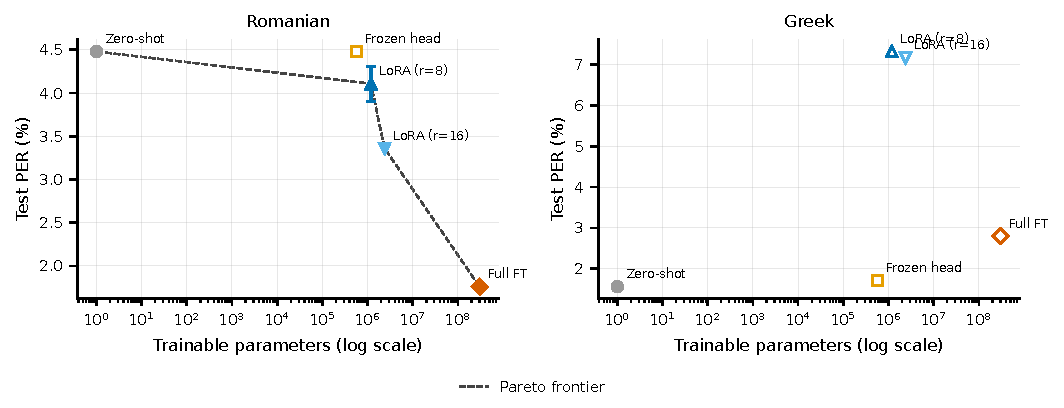
\includegraphics[width=\textwidth]{../figures/fig1_pareto}
\caption{Accuracy--cost trade-off: test PER (\%, lower is better) versus the number of trainable parameters (log scale), per language. Zero-shot is plotted at the cheap extreme (no trainable parameters). Points on the lower-left Pareto frontier dominate. For Romanian, increasing the budget monotonically reduces PER, with full fine-tuning best; for Greek, no fine-tuned configuration improves on the zero-shot point.}
\label{fig:pareto}
\end{figure*}

\begin{figure}[t]
\centering
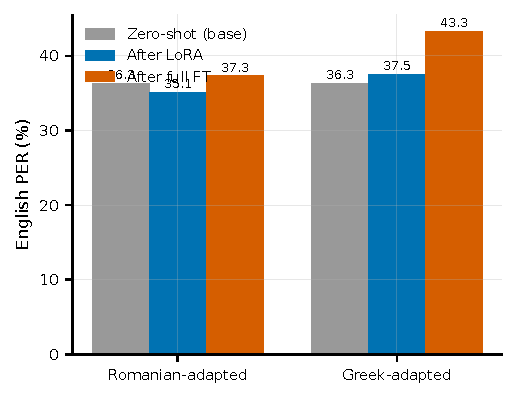
\includegraphics[width=\columnwidth]{../figures/fig2_forgetting}
\caption{Catastrophic forgetting on English (\texttt{eng-us}), measured as character-level PER (\%) after adaptation, grouped by the language each model was adapted to; higher means more forgetting. The unadapted base model scores PER~36.28. Full fine-tuning degrades English the most, while LoRA and the frozen-head baseline stay near the unadapted level.}
\label{fig:forgetting}
\end{figure}

\subsection{Accuracy of the adaptation strategies}

Table~\ref{tab:main} reports the main results. The two languages behave qualitatively differently. For Romanian, adaptation clearly helps: moving from zero-shot (PER~4.48, WER~22) to LoRA $r{=}16$ (PER~3.36, WER~15) and then to full fine-tuning (PER~1.76, WER~10) yields a monotone improvement, and full fine-tuning matches the reported SIGMORPHON~2021 low-resource baseline WER of $\sim$10\%~\cite{ashby2021}. LoRA $r{=}8$ improves over zero-shot on average (PER~$4.11\pm0.20$, WER~$18.67\pm2.36$), and increasing the rank to $16$ closes much of the remaining gap to full fine-tuning. The frozen-head baseline, which adapts only the output projection, leaves PER unchanged (4.48) and slightly worsens WER (23), indicating that for Romanian the useful adaptation lies inside the encoder--decoder attention rather than in the LM head alone.

For Greek the picture is reversed. The zero-shot model is already excellent (PER~1.56, WER~10) and \emph{none} of the fine-tuned configurations improves on it. Full fine-tuning degrades to PER~2.80 (WER~16), and both LoRA ranks are markedly worse (PER~7.17--7.32, WER~35). The frozen-head baseline is the closest to zero-shot (PER~1.71, WER~11) but still does not beat it. This pattern, where additional supervision hurts a model that is already near-optimal on the target distribution, strongly suggests that the Greek zero-shot number reflects prior exposure rather than genuine low-resource generalization; we return to this in the threats to validity.

\subsection{Efficiency and the accuracy--cost trade-off}

Table~\ref{tab:efficiency} quantifies the cost of each strategy. The frozen-head baseline trains only 565{,}248 parameters (0.19\% of the base), and the two LoRA configurations train 1{,}187{,}840 (0.39\%) and 2{,}375{,}680 (0.78\%) parameters respectively, against the 300{,}768{,}256 parameters (100\%) updated by full fine-tuning. In practical terms, PEFT reduces per-language storage from $\sim$300M weights to $\sim$1--2M, roughly a $100$--$250\times$ reduction in the per-language adaptation footprint. Training times are all within the same order of magnitude (hundreds of seconds on dual~T4 GPUs) and are dominated by early stopping and per-language data rather than by the number of trainable parameters; the absolute numbers should therefore be read as indicative rather than as a controlled timing benchmark.

Fig.~\ref{fig:pareto} plots PER against trainable parameters on a log axis. For Romanian the strategies trace a clean Pareto frontier: each increase in budget buys lower PER, so the choice is an explicit accuracy-versus-cost decision, with LoRA $r{=}16$ offering most of the benefit at $0.78\%$ of the parameters and full fine-tuning purchasing the last increment at $130\times$ the cost. For Greek the frontier collapses to the zero-shot point, which dominates every trained alternative, so no point on the parameter axis is worth paying for.

\subsection{Catastrophic forgetting}

Fig.~\ref{fig:forgetting} reports English (\texttt{eng-us}) character-level PER after adapting to each language, relative to the unadapted base model (PER~36.28). Full fine-tuning is by far the most destructive: the Greek-adapted model degrades to PER~43.33 ($+7$ absolute over the unadapted baseline) and the Romanian-adapted model to PER~37.33. In contrast, the PEFT strategies stay near the baseline and in some cases slightly below it: Romanian-adapted LoRA $r{=}16$ reaches PER~35.11 and Greek-adapted frozen-head reaches PER~35.63. Because LoRA leaves the base weights frozen and adds only low-rank updates to the attention projections, the multilingual capability encoded in those base weights is preserved, whereas full fine-tuning overwrites it. This is the cleanest argument in favor of PEFT in our study: even where full fine-tuning wins on the target language (Romanian), it does so at a measurable cost to the model's other languages, while LoRA captures most of the target-language gain without that collateral damage.

\subsection{Discussion}

\textbf{Did LoRA match full fine-tuning?} Partially, and in a language-dependent way. For Romanian, full fine-tuning remains the most accurate strategy (PER~1.76), but LoRA $r{=}16$ recovers a large fraction of the improvement over zero-shot (PER~$4.48\rightarrow3.36$) while updating under~$1\%$ of the parameters and without the forgetting penalty, making it an attractive operating point when the multilingual base must be preserved. For Greek, the question is moot: neither LoRA nor full fine-tuning beats zero-shot, so the appropriate choice is to not adapt at all. LoRA thus does not uniformly match full fine-tuning, but it offers a favorable accuracy-per-parameter and accuracy-per-side-effect trade-off wherever adaptation is warranted.

\textbf{Does the script or branch difference matter?} The two target languages use different scripts (Latin for Romanian, Greek for Greek) but our findings do not appear to be driven by orthography. The divergent behavior is better explained by the base model's prior competence on each language than by script: Greek zero-shot is already near-perfect, leaving no room for the small training set to help, whereas Romanian zero-shot has clear headroom that adaptation fills. We therefore attribute the contrast to pretraining coverage rather than to a script or branch effect, and we validated that correct language tagging is essential in any case: using the correct ISO~639-3 tag \texttt{<ron>} for Romanian yields a zero-shot dev PER of 5.96\% versus 24.76\% with the incorrect \texttt{<rum>} code, a $4\times$ difference driven entirely by tag selection.

\textbf{Is forgetting alone enough to justify PEFT?} For a single-language deployment where the base model will only ever serve one language, the forgetting result is not decisive on its own, since the degraded English performance is irrelevant to that use case and full fine-tuning gives the best Romanian accuracy. The argument becomes compelling in the realistic multilingual setting that CharsiuG2P targets: there, a shared base must remain competent across many languages simultaneously, and full fine-tuning's $+7$-point English degradation (Greek-adapted) is unacceptable, whereas LoRA's per-language adapters can be swapped in without touching the base. Combined with the $100$--$250\times$ storage reduction, forgetting tips the balance toward PEFT for multilingual G2P deployment.

\textbf{Limitations.} This is a methodological study on a deliberately narrow slice of the problem, and several limitations bound its conclusions. We study only two languages and two LoRA ranks ($r\in\{8,16\}$); most configurations use a single seed (42), with three seeds only for the headline Romanian LoRA $r{=}8$ setting, so per-configuration variance is largely uncharacterized and the single-seed numbers should be read with corresponding caution. We use a single base model (\texttt{charsiu/g2p\_multilingual\_byT5\_small}) and evaluate isolated words only, with no sentence- or context-level G2P. Finally, we compare LoRA against full fine-tuning and simple baselines but do not include bottleneck adapter modules~\cite{houlsby2019}, which would sharpen the PEFT comparison; we leave a broader sweep over ranks, seeds, adapter families, base models, and languages to future work.

\textbf{Threats to validity.} Two threats deserve emphasis. First, the Greek zero-shot result is most plausibly explained by overlap between CharsiuG2P's WikiPron-derived pretraining and the SIGMORPHON Greek data, which would inflate the apparent zero-shot quality and explain why supervised adaptation cannot improve on it. Importantly, this leakage is \emph{not} within the SIGMORPHON splits themselves: we measured 0\% exact word overlap and 0\% exact (grapheme, phoneme) pair overlap between train and test for both languages, with only 28\%/15\% (Romanian/Greek) of test words sharing a $\geq$4-character substring with a training word. The likely overlap is therefore between the pretraining corpus and the evaluation set, a genuine threat to the external validity of the Greek zero-shot number that we cannot fully rule out without access to the exact pretraining data. Second, our PER is a micro-averaged \emph{character-level} edit rate, computed with phoneme delimiters removed, because the pretrained model emits un-delimited IPA (e.g.,~\ipa{aŋɟelos}) whereas the SIGMORPHON gold and the fine-tuned models use space-separated phonemes; without this normalization a phonetically correct zero-shot prediction would be scored as 100\% error. As a consequence our absolute PER is not strictly comparable to the official SIGMORPHON phoneme-token PER~\cite{gorman2020,ashby2021}, and we report it only for internal comparison across our own configurations; for the delimited fine-tuned outputs our WER is equivalent to the official exact-match WER, so WER comparisons to the baseline are sound. In light of these threats, we frame our contribution as a methodological comparison of parameter-efficient adaptation strategies for multilingual G2P, not as a claim of state-of-the-art accuracy.

\section{Conclusion}\label{sec:conclusion}

We presented a methodological study of parameter-efficient adaptation for multilingual grapheme-to-phoneme conversion, comparing zero-shot inference, a trainable LM head, LoRA~\cite{hu2021}, and full fine-tuning of the ByT5-based CharsiuG2P model~\cite{zhu2022,xue2022byt5} on the low-resource Romanian and Modern Greek subtasks of SIGMORPHON 2021~\cite{ashby2021}. The picture differs sharply by language. On Romanian, adaptation clearly helps: LoRA $r{=}16$ reaches PER~3.36 while training only 0.78\% of the parameters, beating zero-shot (PER~4.48), and full fine-tuning is best at PER~1.76 / WER~10, matching the SIGMORPHON baseline WER. On Greek, zero-shot is already excellent (PER~1.56) and fine-tuning does not improve it, most plausibly because the WikiPron-based pretraining overlaps the test data---a genuine threat to validity rather than a property of the method. Finally, full fine-tuning incurs the most catastrophic forgetting on held-out English (Greek-adapted PER~43.3 vs.\ the 36.3 baseline), whereas LoRA and the frozen-head variant stay near baseline.

These results argue for PEFT as a practical default for per-language G2P deployment. LoRA matches or approaches full fine-tuning where adaptation is warranted while training under 1\% of the weights, so storing $K$ specialized languages drops from $K\times{\sim}300$M to $K\times{\sim}1$--$2$M parameters. Just as importantly, by leaving the backbone frozen, LoRA preserves the multilingual base and avoids the destructive interference that full fine-tuning causes on unrelated languages, making it well suited to incremental, multi-language rollout from a single shared model.

Several directions remain open. A broader exploration of the design space---adapter modules~\cite{houlsby2019} and a larger LoRA-rank sweep---would sharpen the accuracy/efficiency trade-off, as would extending the study to more languages and writing scripts. Combining PEFT with self-training~\cite{vesik2020} could further exploit unlabeled lexicons in genuinely low-resource settings, and moving from isolated words to sentence-level G2P would require homograph disambiguation. Finally, pairing PEFT with robustness-oriented methods such as r-G2P~\cite{zhao2022} is a promising route to adapted models that remain resilient to noisy input.

\bibliographystyle{IEEEtran}
\bibliography{references}

\end{document}
